\NewScheme{\SPOR}{SPOR}
\NewScheme{\POR}{POR}

\subsection{\Acfp*{SPOR}}%
\label{sec:message_passing}

\NewAlgorithm{\Send}{Send}
\NewAlgorithm{\Fwd}{Forward}
\NewAlgorithm{\Recv}{Receive}
\NewVariable{\rdv}{rdv}

We now describe a protocol \ac{SPOR}, which uses the \ac{POR} of Sphinxes to 
transfer large messages from a source to a destination.
We provide the following algorithms:
\begin{itemize}
  \item \(\SPOR[\Send]\) (\cref{SPORSend}).
  \item \(\SPOR[\Fwd]\) (\cref{SPORFwd}).
  \item \(\SPOR[\Recv]\) (\cref{SPORRecv}).
\end{itemize}

Say that Alice wants to send a message \(m\) to Bob.
Bob runs the \(\SPOR[\Recv]\) algorithm and Alice runs the \(\SPOR[\Send]\) 
algorithm.
Bob (\ie \(\SPOR[\Recv]\)) creates a reply header using \(\CreateRe\) and gives 
the output to Alice (\ie \(\SPOR[\Send]\)) out-of-band.
At a later point, Alice creates a forward header using \(\CreateFwd\), attaches 
the message \(m\) as payload and sends the package to the first node, \ie 
invokes the \(\SPOR[\Fwd]\) algorithm on the first node (\eg as a remote 
procedure call).
The node will then process the package and in turn forward the package to the 
next node, if itself is not the final destination.

\NewAlgorithm{\Store}{Store}
\NewAlgorithm{\Dec}{Dec}
\NewVariable{\sk}{sk}

\begin{figure}
  \framebox{\begin{minipage}{0.96\linewidth}
  \begin{algorithmic}
    \Require{%
      $D$ is the set of alternative recipient devices.
    }
    \Function{\POR[\Recv]}{$D$}
      \State $H_\rdv\gets \ExtendRoute[D\concat \top, L, \theta]$
      \State \Return $H_\rdv$
        \Comment{Give to sender out-of-bound.}
    \EndFunction
  \end{algorithmic}
  \end{minipage}}
  \caption{\label{SPORRecv}%
    The \(\POR[\Recv]\) algorithm prepares the recipient for receiving a file.
    It creates a probabilistic onion-route from a rendez-vous point to its own 
    devices and returns the route to the sender.
  }
\end{figure}

\begin{figure}
  \framebox{\begin{minipage}{0.96\linewidth}
  \begin{algorithmic}
    \Require{%
      $m$ is the message to be sent,
      $H_\rdv$ is the onion-route given by the recipient.
    }
    \Function{\POR[\Send]}{$H_\rdv, m$}
      \State $H\gets \ExtendRoute[H_\rdv, L, \theta]$
      \State $D\concat C_H\gets H_\rdv$
      \For{$d\in D$}
        \Comment{Uniformly randomly chosen}
        \If{$d\method \Fwd[C_H, m] \neq \bot$}
          \State \Return $\top$
        \EndIf
      \EndFor
      \State \Return $\bot$
    \EndFunction
  \end{algorithmic}
  \end{minipage}}
  \caption{\label{SPORSend}%
    The \(\POR[\Send]\) algorithm extends the route \(H_\rdv\) (using 
    \(\ExtendRoute\), \cref{ExtendRoute}) and sends the message \(m\) down the 
    extended route using the \(\POR[\Fwd]\) algorithm (\cref{SPORFwd}).
    The first node of \(H_\rdv\) is the rendez-vous point selected by the 
    recipient.
  }
\end{figure}

\begin{figure}
  \framebox{\begin{minipage}{0.96\linewidth}
  \begin{algorithmic}
    \Require{$\pk, \sk$ is the public--private key-pair of the node.}
    \Function{\POR[\Fwd]}{$C_H, m$}
      \State $H\gets \DeBEdec[\mpk, \sk, C_H]$
      \If{$H = \bot$}
        \State \Return $\bot$
      \EndIf
      \State $\{d_i\}\concat C_H'\gets H$
      \If{$C_H' = \top$}
        \State \Return $\Store[m]$
      \EndIf
      \For{$d\in \{d_i\}$}
        \Comment{Uniformly randomly chosen}
        \If{$d\method \Fwd[C_H', m] \neq \bot$}
          \State \Return $\top$
        \EndIf
      \EndFor
      \State \Return $\bot$
    \EndFunction

    \Function{\Store}{$m$}
      \State $m\gets \DeBEdec[\mpk, \sk, c_m]$
      \If{$m = \bot$}
        \State \Return $\bot$
      \EndIf
      \State Store $m$ to disk.
      \State \Return $\top$
    \EndFunction
  \end{algorithmic}
  \end{minipage}}
  \caption{\label{SPORFwd}%
    The \(\POR[\Fwd]\) algorithm forwards \(m\) down the route \(H\), obtained 
    by decrypting \(C_H\) with the node's associated private key.
    The special value \(H = \top\) indicated the end of the route, thus \(c_m\) 
    is intended for the local node and \(c_m\) is instead sent to disk using 
    \(\Store\).%
  }
\end{figure}

\subsection{\Acf*{SPORES}}

\dots

To create a probabilistic onion route \(H_\rdv\) from a rendez-vous point to 
his own device swarm --- all the hops on the route are chosen by Bob uniformly 
at random.
Bob gives \(H_\rdv\) to Alice using an out-of-band channel, \eg using his phone.
Alice uses \(\SPOR[\Send]\) at some later time to send the message to Bob using 
any of her devices.
\(\SPOR[\Send]\) extends the route \(H_\rdv\) with some hops of Alice's 
choosing (uniformly randomly chosen), then starts to forward the message (using 
\(\SPOR[\Fwd]\)) through the hops on the route to Bob.
This process is illustrated in \cref{fig:file-exchange}.

\begin{figure}
  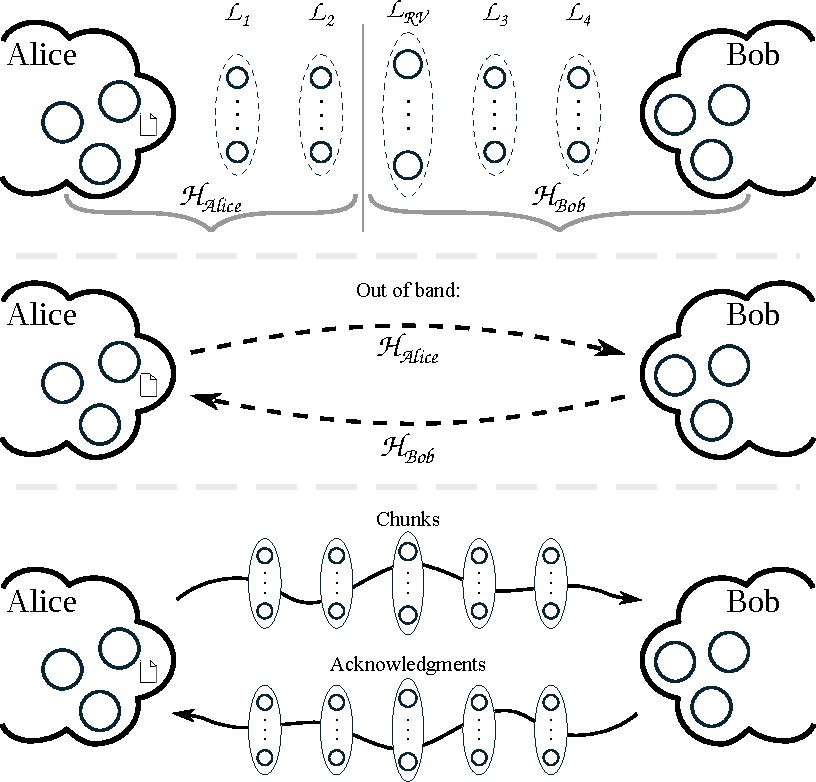
\includegraphics[width=\linewidth]{figures/file_exchange_v2.pdf}
  \caption{\label{fig:file-exchange}%
    A schematic of Alice and Bob sending a message using \(\SPORES\).
    \ding{1} illustrates the layer of the headers that Alice and Bob create.
    In \ding{2}, Alice and Bob exchange the headers out-of-band.
    In \ding{3}, Alice and Bob use two \ac{SPOR} routes, one for messages and 
    one for acknowledgements.
  }
\end{figure}

